\documentclass[12pt,a4paper]{article}
\usepackage{listings}
% ----------------- Paquetes -----------------
\usepackage[utf8]{inputenc}
\usepackage[spanish]{babel}
\usepackage[a4paper,top=2.5cm,bottom=2.5cm,left=3cm,right=3cm]{geometry}
\usepackage{setspace}
\usepackage{graphicx}
\usepackage{amsmath}
\usepackage{titlesec}
\usepackage{url}
\usepackage{enumitem}
\usepackage{multicol}
\usepackage{helvet} % Arial-like font
\usepackage{comment}
\usepackage{caption}
\usepackage{indentfirst}
% ----------------- Fuente Arial -----------------
\usepackage{fancyhdr} % Encabezado y pie de página
\renewcommand{\familydefault}{\sfdefault}
% ----------------- Fuente Arial -----------------

% ----------------- Interlineado 1.5 -----------------
\onehalfspacing

% ----------------- Espaciado de párrafo (0 pt antes/después) -----------------
\setlength{\parskip}{0pt}

% ----------------- Sangría de 0.5 cm al inicio de sección/subsección -----------------
\setlength{\parindent}{0.5cm}

% ----------------- Estilos de sección -----------------
\titleformat{\section}{\bfseries\fontsize{14}{16}\selectfont}{\thesection}{1em}{}
\titleformat{\subsection}{\bfseries\fontsize{12}{14}\selectfont}{\thesubsection}{1em}{}

% ----------------- Nombre de Tabla en español -----------------
\addto\captionsspanish{\renewcommand{\tablename}{Tabla}}

% ----------------- Formato de títulos de figuras y tablas -----------------
% Arial 11, sin dos puntos, centrado. El punto final se escribe a mano
% en cada \caption{...}: con format=puntofinal el punto se colocaba fuera
% del bloque centrado del caption y aparecía huérfano en su propia línea.
\DeclareCaptionFont{arial11}{\fontsize{11}{13}\selectfont}
\captionsetup{
  font=arial11,
  labelfont=arial11,
  labelsep=space,
  justification=centering,
  singlelinecheck=false
}

% ----------------- Nota de fuente (Arial 9, cursiva, alineada a la derecha) -----------------
\newcommand{\fuente}[1]{\par\vspace{2pt}{\setstretch{1.15}\raggedleft\fontsize{9}{11}\selectfont\itshape Fuente: #1\par}\vspace{4pt}}

% ----------------- Pie de página -----------------
    
\pagestyle{fancy}
\fancyhf{} % Limpia encabezados y pies
\begin{comment}
\fancyfoot[L]{\fontsize{10}{12}\selectfont Circuitos Eléctricos de CA, IE-AD25}
\fancyfoot[R]{\fontsize{10}{12}\selectfont Dr. Luis Alejandro Flores Oropeza}
\end{comment}

\renewcommand{\headrulewidth}{0pt} % sin línea en encabezado
\renewcommand{\footrulewidth}{0pt} % sin línea en pie de página

%-- Das comm --
\newcommand{\titulos}[3]{
  {\fontsize{12}{14}\bfseries \textit{#1}}\\
  {\fontsize{10}{12}\normalfont #2}\\
  {\fontsize{9}{11}\itshape #3}\\[0.5cm]

}
\usepackage{graphicx}
\usepackage{float} % permite [H]: figuras en línea con el texto, sin flotar

\begin{document}

\begingroup
\setstretch{1.15}
\begin{center}
  {\fontsize{16}{18}\bfseries \MakeUppercase{Desarrollo asistido por Inteligencia Artificial de un resolvedor de sistemas de ecuaciones complejas para análisis de circuitos}}\\[0.5cm]
  {\fontsize{14}{16}\itshape \MakeUppercase{AI-Assisted Development of a Complex System Solver for Circuit Analysis}}\\[1cm]

    \titulos{Orlando Contreras Reyes}{Universidad Autónoma de Aguascalientes}{al348390@edu.uaa.mx}

    \titulos{Iker Emiliano García Barrera}{Universidad Autónoma de Aguascalientes}{al307630@edu.uaa.mx}

    \titulos{Dr. Luís Alejandro Flores Oropeza}{Universidad Autónoma de Aguascalientes}{alejandro.floreso@edu.uaa.mx}

    \titulos{Dr. Alejandro Román Loera }{Universidad Autónoma de Aguascalientes}{ alejandro.roman@edu.uaa.mx}

\end{center}
\endgroup

\section*{Resumen}

Como proyecto integrador, se desarrolló una calculadora capaz de resolver sistemas de ecuaciones con números complejos, con el objetivo de facilitar los cálculos en métodos de análisis de circuitos como mallas o nodos.
El programa se implementó en Python utilizando diversas librerías especializadas, con apoyo de herramientas de inteligencia artificial para acelerar el desarrollo. Además, se compiló como un ejecutable con interfaz gráfica compatible con los sistemas operativos Windows y GNU/Linux. La calculadora permite visualizar los resultados de forma clara e intuitiva para el usuario.

\noindent \textbf{Palabras clave:} Calculadora, Manual, Números complejos, Python, Sistema de ecuaciones.

\section*{\itshape Abstract}
\textit{
As an integrative project, a calculator was developed to solve systems of equations with complex numbers, with the goal of facilitating calculations in circuit analysis methods such as mesh and nodal analysis. The program was developed in Python using various specialized libraries and with the support of AI tools to accelerate development. It was implemented as an executable with a graphical user interface compatible with Windows and GNU/Linux. The calculator allows users to visualize results in a clear and intuitive manner.
}

\noindent \textit{\textbf{Keywords:} Calculator, Complex numbers, Manual, Python, System of equations.}

\section{Introducción}
El análisis de circuitos es una de las tareas más importantes para un ingeniero, implica aplicar conceptos matemáticos y físicos para obtener parámetros como el voltaje o la corriente en un circuito. El análisis de circuitos es una aplicación directa de la ingeniería y gracias a él está formada la tecnología actual. Sin el análisis de circuitos no sería posible construir los dispositivos y las comodidades que se presentan en nuestro día a día. \\

% TODO: sustituir por la imagen real del método de mallas / LVK
% \begin{figure}[!h]
%     \centering
%     \includegraphics[width=0.6\linewidth]{ruta/a/imagen_metodo.png}
%     \fuente{elaboración propia}
%     \caption{Análisis de una trayectoria cerrada mediante la Ley de Voltajes de Kirchhoff}
%     \label{fig:metodo_lvk}
% \end{figure}
\begin{comment}

Otro concepto importante en la actualidad es la distinción entre corriente alterna y corriente directa. Mientras que la corriente alterna es la corriente utilizada para alta potencia y para la alimentación de electrodomésticos o de uso diario, la corriente directa es aquella que utilizan las baterías para almacenar carga. La gran diferencia entre ambas radica en su comportamiento a través del tiempo: mientras que la corriente directa permanece invariable en el tiempo, la corriente alterna es una corriente que oscila de forma senoidal. Para poder analizar este comportamiento con facilidad, los matemáticos introducen el concepto de ondas temporales y, con ello, el término de fasores y números complejos, siendo estas herramientas las que facilitan la manipulación aritmética. \\
\end{comment}

Se reitera el concepto de practicidad y herramientas, pues en la labor del ingeniero es fundamental resolver problemas de forma eficiente. Es aquí donde entra el concepto de calculadora, una herramienta que permite la resolución de problemas matemáticos de forma eficiente. El ingeniero debe ser capaz, entonces, de crear herramientas que faciliten estos procesos. El problema que suele ocurrir con esta filosofía es la nula aplicación en el aula. En este caso, el problema que se abordó fue la necesidad de una solución para resolver circuitos de CA de forma efectiva y portátil. Las soluciones que han surgido a lo largo de los años para este problema son las siguientes:

\begin{itemize}
    \item Comprar una calculadora específica que permita resolver este tipo de sistemas de ecuaciones complejas.
    \item Utilizar simuladores de calculadoras en el celular.
    \item Utilizar métodos de resolución, como la regla de Cramer, y aplicarlos manualmente.
\end{itemize}

La calculadora que usualmente se simulaba era la HP 48G tal y como se ve en la imagen \ref{fig:HP48} y su version en aplicacion \ref{fig:Droid48}, como se puede ver es una calculadora bastante robusta y con multiples funciones, además teniendo botones que siempre están ahi a pesar de no ser utiles para lo que se esta haciendo.
\begin{figure}[!h]
    \centering
    \begin{minipage}[b]{0.48\linewidth}
        \centering
        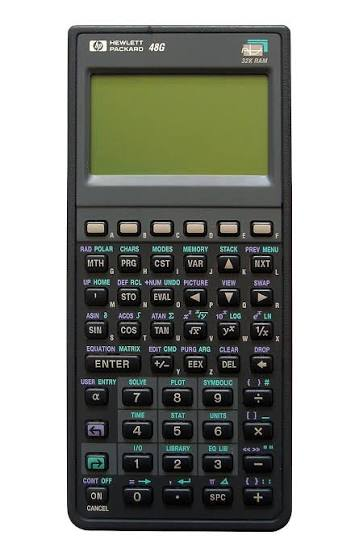
\includegraphics[width=1\linewidth]{../src/Hp48G.png}
        \fuente{Wikipedia/HP-48}
        \caption{Calculadora HP-48}
        \label{fig:HP48}
    \end{minipage}
    \hfill % Espacio horizontal automático entre las minipáginas
    \begin{minipage}[b]{0.48\linewidth}
        \centering
        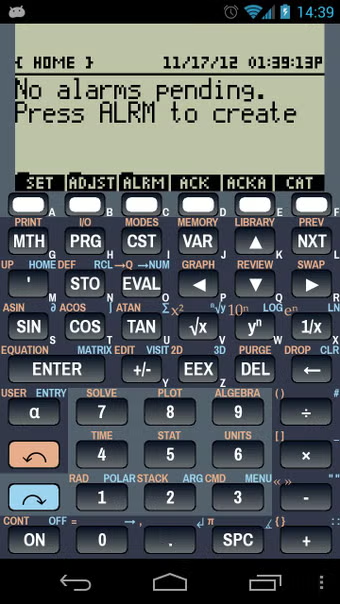
\includegraphics[width=.8\linewidth]{../src/Droid48.png}
        \fuente{Google Play Store/Droid 48}
        \caption{Droid 48}
        \label{fig:Droid48}
    \end{minipage}
\end{figure}

Los problemas encontrados en estas soluciones fueron los siguientes:

\begin{itemize}
    \item Regla de Cramer: método poco eficiente.
    \item Simuladores de calculadoras y calculadoras físicas: método de ingreso de datos poco eficiente, y obtención de resultados solo en forma rectangular o solo en forma polar.
    \item Deshonestidad académica Uso de calculadoras o simuladores para resolver de forma deshonesta, apoyándose en IA o en compañeros de clase, sin comprender el proceso. \\
\end{itemize}
Como se puede ver en la figura \ref{fig:interfazfea} la interfaz es poco amigable para el usuario, no se consigue aprovechar el tamaño de la pantala dejandolo en una cantidad de celdas fijas y estatica. \\


\begin{figure}[!h]
    \centering
    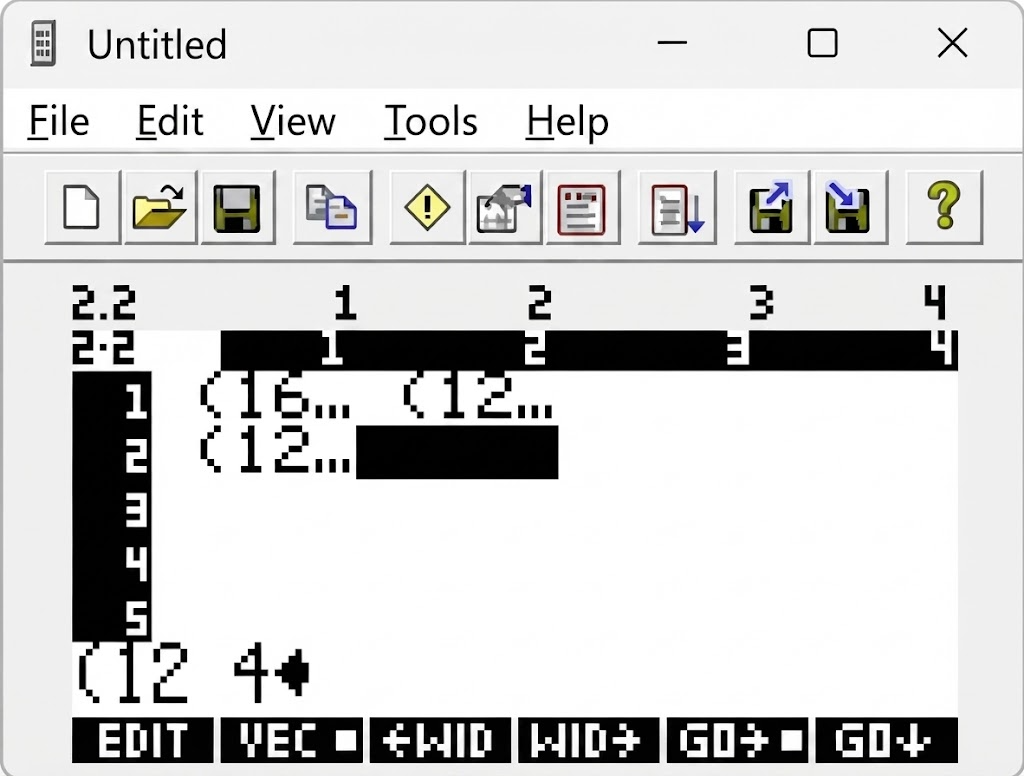
\includegraphics[width=0.6\linewidth]{../src/Droid48PC.png}
    \caption{Solución de ecuaciones por medio de Droid48}
    \fuente{elaboración propia}
    \label{fig:interfea}
\end{figure}
%https://youtu.be/7VeAC4dk9nY?si=t3peVqy3xGbsoB7F
Es por ello que un equipo de estudiantes se dedicó a atender estas problemáticas directamente mediante la creación de una aplicación de escritorio, empaquetada en un ejecutable (.exe) como primer prototipo, para después implementarla como aplicación de Android y una versión en hardware. \\

Cabe destacar que el primer prototipo (.exe) fue diseñado en conjunto con la IA. Es importante destacar esto, pues demuestra el alcance de un ingeniero electrónico apoyado en inteligencia artificial:

\section{Métodos}

Para el desarrollo del proyecto se adoptó un enfoque metodológico dividido en tres fases principales: la selección de herramientas y arquitectura del software, la implementación de los algoritmos matemáticos en conjunto con el flujo de trabajo apoyado por Inteligencia Artificial, y la construcción de la interfaz gráfica junto con su posterior empaquetado ejecutable.
\subsection{Materiales y Herramientas}
\begin{itemize}
    \item \textbf{Entorno de desarrollo:} Visual Studio Code v1.85+.
    \item \textbf{Lenguaje de programación:} Python 3.10+.
    \item \textbf{Librerías principales:}
    \begin{itemize}
        \item \texttt{NumPy}: Manipulación de matrices y resolución de sistemas de ecuaciones lineales complejas mediante álgebra lineal numérica.
        \item \texttt{CustomTkinter} y \texttt{Tkinter}: Creación y personalización de la interfaz gráfica de usuario (GUI) moderna.
        \item \texttt{Pillow (PIL)}: Procesamiento y renderizado de recursos gráficos dentro de la interfaz.
        \item \texttt{OS} y \texttt{JSON}: Gestión de archivos del sistema, persistencia de datos e importación/exportación de historiales de matrices.
    \end{itemize}
    \item \textbf{Herramientas de IA:} Asistente de código basado en el modelo ChatGPT (OpenAI), empleado para optimización de fragmentos de código, refactorización y aceleración en el diseño de componentes GUI.
    \item \textbf{Herramienta de compilación:} \texttt{PyInstaller}, para empaquetar el script de Python en un ejecutable binario autónomo (\texttt{.exe}).
\end{itemize}

\begin{figure}[h]
    \centering
    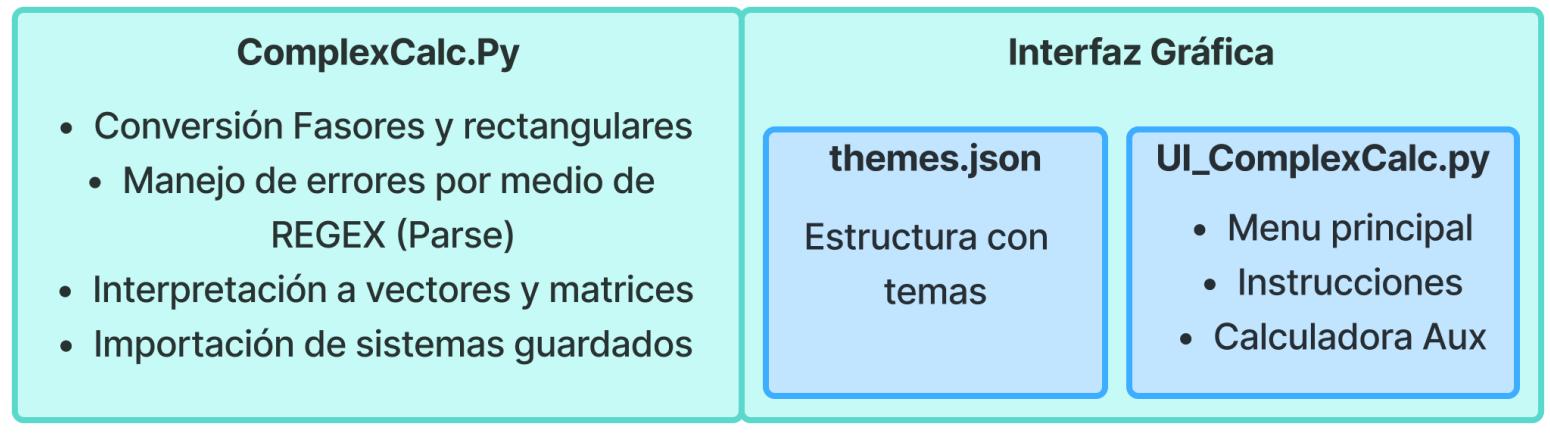
\includegraphics[width=\linewidth]{../src/Architecture.png}
    \caption{Arquitectura}
    \fuente{Elaboracion propia}
    \label{fig:placeholder}
\end{figure}
\subsection{Arquitectura del Software y Algoritmos Matemáticos}
La herramienta está estructurada bajo una arquitectura modular dividida en lógica matemática, interfaz de usuario y gestión de datos:

\begin{enumerate}
    \item \textbf{Procesamiento e ingreso de datos complejos:} Se diseñó un módulo capaz de recibir datos tanto en forma rectangular ($a + jb$) como polar ($r\angle\theta^\circ$).

    \item \textbf{Resolución del sistema de ecuaciones:} Un sistema de mallas o nodos de $n \times n$ se representa matricialmente como:
    \begin{equation}
        [\mathbf{Z}] [\mathbf{I}] = [\mathbf{V}] \quad \implies \quad [\mathbf{I}] = [\mathbf{Z}]^{-1} [\mathbf{V}]
    \end{equation}
    donde $[\mathbf{Z}]$ es la matriz de impedancias complejas, $[\mathbf{I}]$ el vector de corrientes desconocidas y $[\mathbf{V}]$ el vector de fuentes. La resolución se realiza invocando el solver numérico de \texttt{NumPy} (\texttt{numpy.linalg.solve}), garantizando alta precisión decimal y eficiencia computacional frente al uso tradicional de la regla de Cramer.

    \item \textbf{Conversión y renderizado de resultados:} Una vez calculado el vector solución, la herramienta convierte automáticamente cada componente a su forma polar ($r = \sqrt{a^2 + b^2}, \; \theta = \arctan(b/a)$) para presentar al usuario ambos formatos de manera simultánea e intuitiva.
\end{enumerate}

\subsection{Flujo de Trabajo Co-diseñado con Inteligencia Artificial}
El desarrollo del software integró un ciclo iterativo de asistencia con IA (ChatGPT) compuesto por cuatro etapas:
\begin{itemize}
    \item \textbf{Generación de maquetas iniciales:} Solicitud de código base estructurado para ventanas, contenedores dinámicos y celdas matriciales editables.
    \item \textbf{Resolución de limitaciones de componentes:} Solución de errores al manipular arreglos multidimensionales complejos en tiempo real.
    \item \textbf{Refactorización y optimización:} Limpieza del código para separar la lógica de cálculo del renderizado gráfico, mejorando la mantenibilidad.
    \item \textbf{Supervisión y validación humana:} Cada segmento de código generado por la IA fue revisado, adaptado, probado técnicamente y validado contra ejercicios teóricos resueltos manualmente.
\end{itemize}

\subsection{Diseño de la Interfaz Gráfica y Empaquetado}
Para superar el aspecto nativo y limitado de \texttt{Tkinter}, se adoptó \texttt{CustomTkinter} complementado con un archivo de configuración \texttt{.json} para la paleta de colores y estilos visuales. Se incorporó una barra de herramientas con funciones para guardar matrices en disco, limpiar celdas y alternar la visualización del formato de salida. \\

Finalmente, el programa principal se compiló mediante \texttt{PyInstaller} utilizando los parámetros \texttt{--onefile} y \texttt{--noconsole}, empaquetando el intérprete de Python, las dependencias y los recursos estáticos en un solo ejecutable listo para su distribución.

\subsection{Filosofía}
Es importante destacar la filosofía con la que el proyecto se creó siendo la filosofia \textit{Open Source} y \textit{Vibe Coding} dos filosofías aparentemente opuestas pero muy fundamentales en la creación del proyecto. \\


Este mismo busca la mejora a través de la comunidad y la accesibilidad al contribuir, es importante destacar que la creación
del proyecto fue realizada por alumnos que sólo llevaron las bases de programación en C dedicado a microcontroladores, se destaca debido a el enfásis de la filosofía Vibe Coding, logrando que, con buenas bases en programación el ingeniero es capaz de poder construir sus herramientas para resolver necesidades de forma práctica; esta sinergia permite desarrollar prototipos de hardware y software de forma óptima y práctica.Todo esto siguiendo una filosofía open source y open hardware, para facilitar la personalización y una reproducción accesible hacia el rubro que se está atendiendo: los ingenieros del mañana.  \\

\newpage

Parte de la filosofía del proyecto fue desarrollar una solución que pudiera estar disponible rápidamente, que fuera sencilla de utilizar y que, al mismo tiempo, tuviera una base tecnológica que permitiera demostrar su funcionamiento de manera práctica. Por esta razón, se optó por utilizar Python y apoyarse en herramientas de inteligencia artificial durante el proceso de desarrollo, buscando agilizar la implementación sin dejar de lado la funcionalidad del programa. \\

Asimismo, el proyecto se planteó como una forma de contribuir al salón y facilitar determinadas actividades académicas, particularmente durante los periodos de exámenes y en aquellas situaciones en las que una herramienta de este tipo pudiera resultar útil para los estudiantes. \\

De esta manera, el proyecto no se limita únicamente a resolver una necesidad inmediata, sino que busca servir como una base sobre la cual otros estudiantes puedan aprender, contribuir e incluso desarrollar sus propias soluciones. Se pretende que la sencillez del proyecto también pueda servir como inspiración para que más personas se animen a desarrollar herramientas similares y comprueben que la creación de software útil puede comenzar de una manera accesible y sencilla.

\begin{figure}[!h]
    \centering
    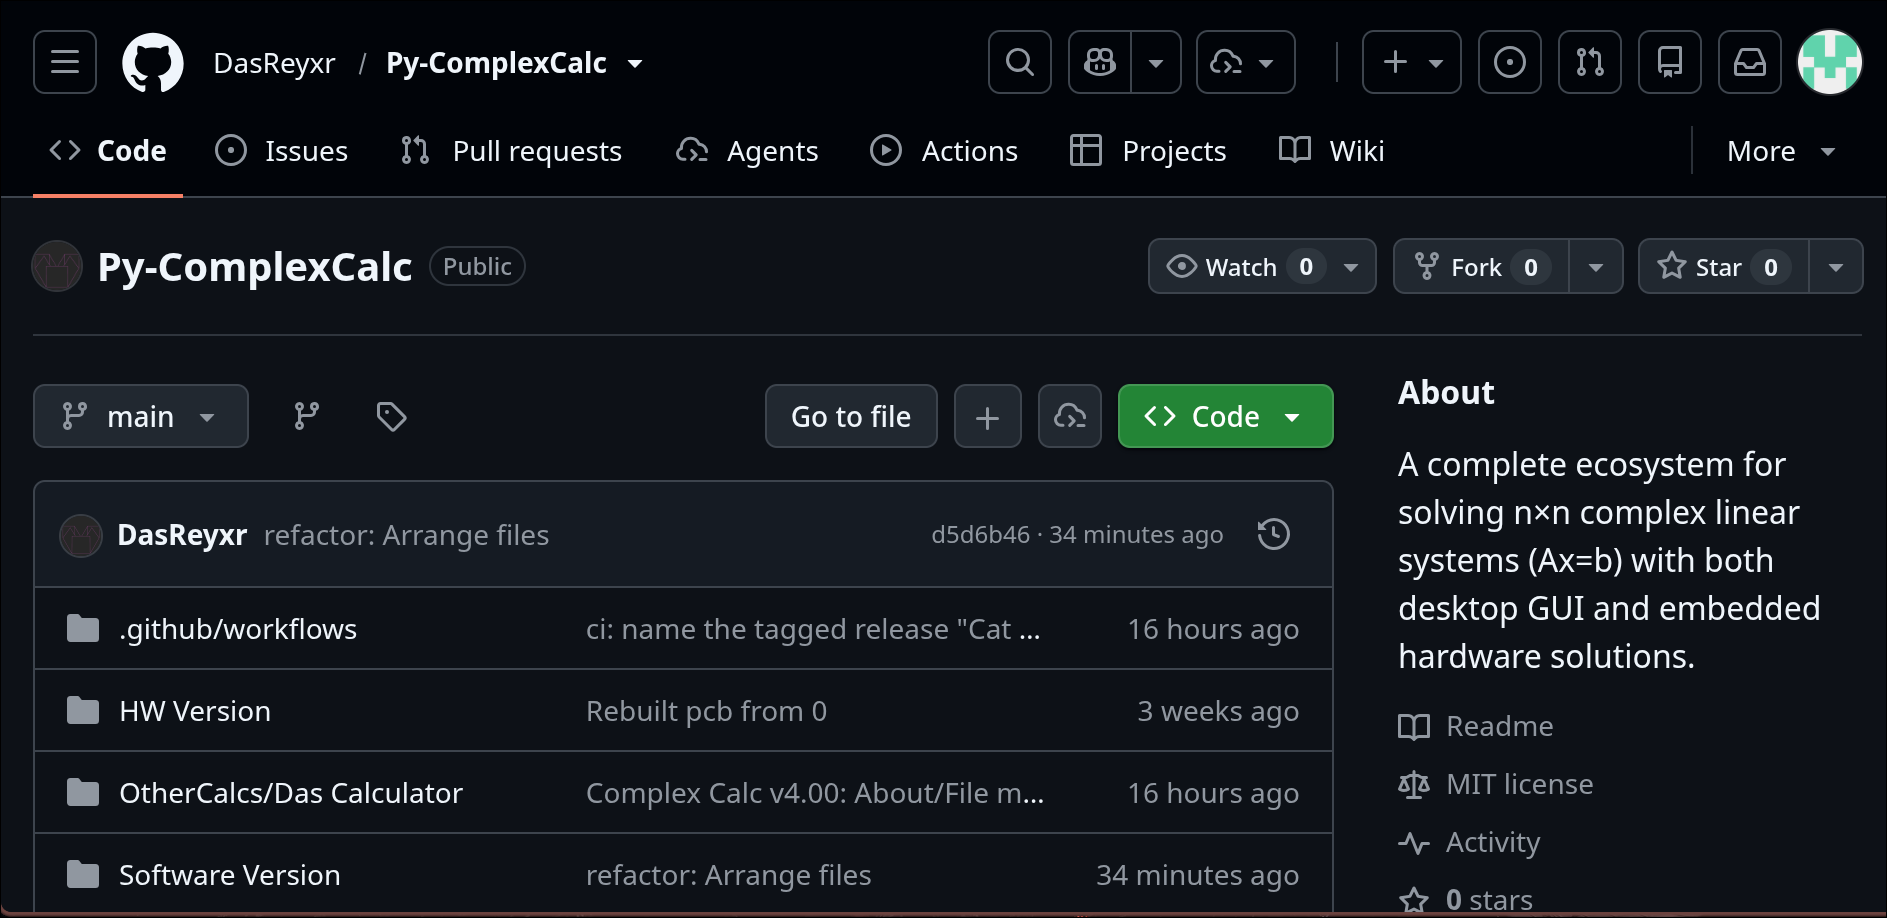
\includegraphics[width=1\linewidth]{../src/Github.png}
    \fuente{Elaboración propia}
    \caption{Repositorio de Github de la calculadora}
    \label{fig:placeholder}
\end{figure}

%{\centering \color{blue} \url{https://github.com/DasReyxr/Py-ComplexCalc/tree/main} \par}

\bigskip
\noindent \textit{\textbf{Aclaración de autoría y licenciamiento:} Parte de las estructuras de código fuente e interfaz fueron desarrolladas con apoyo del modelo de inteligencia artificial ChatGPT. El proyecto se distribuye de manera pública bajo la licencia MIT.}

\newpage

\section{Resultados}

En la Figura~\ref{fig:interfaz2} se muestra la solución obtenida por la calculadora para un sistema de ecuaciones complejas expresado en forma rectangular, donde se observan tanto los valores ingresados como el resultado calculado para cada incógnita.


\begin{figure}[H]
    \centering
    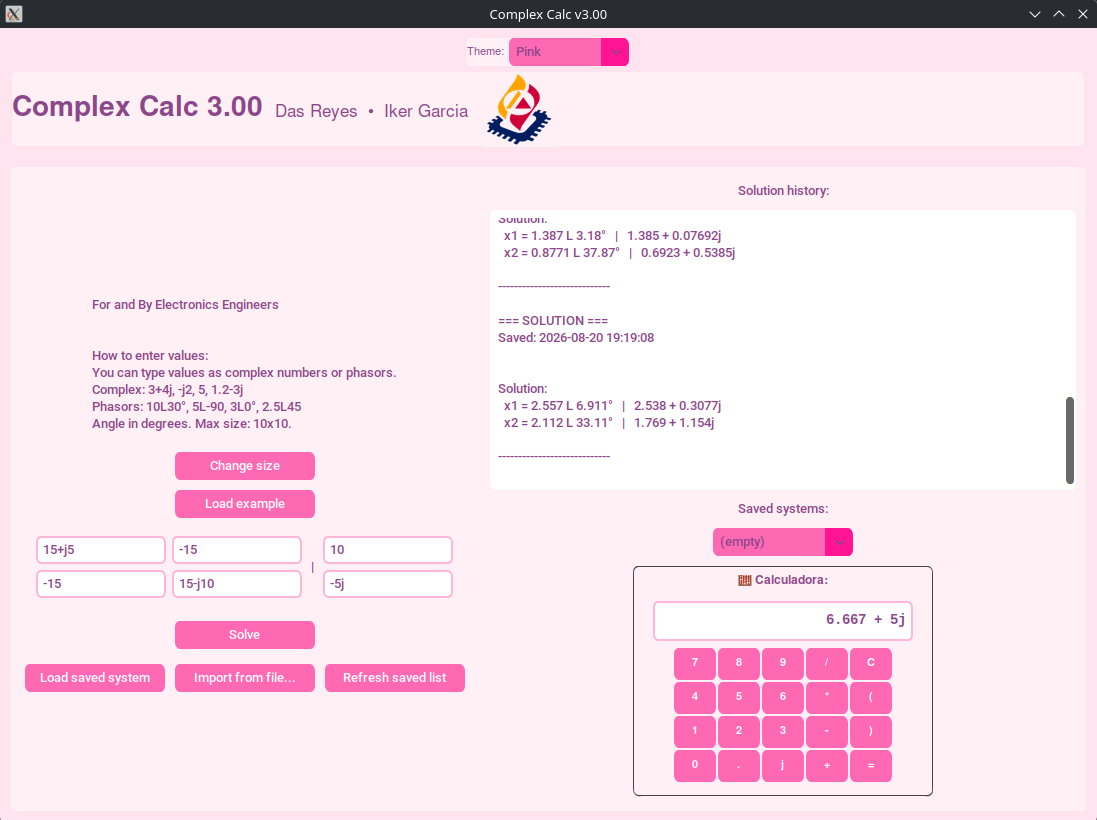
\includegraphics[width=0.68\linewidth]{../src/RectSol.png}
    \fuente{elaboración propia}
    \caption{Solución de un sistema complejo de forma Rectangular.}
    \label{fig:interfaz2}
\end{figure}

En la Figura~\ref{fig:interfaz4} se presenta una ecuación expresada en forma polar, lo que permite comprobar la conversión automática entre ambas representaciones que realiza la herramienta.



\begin{figure}[H]
    \centering
    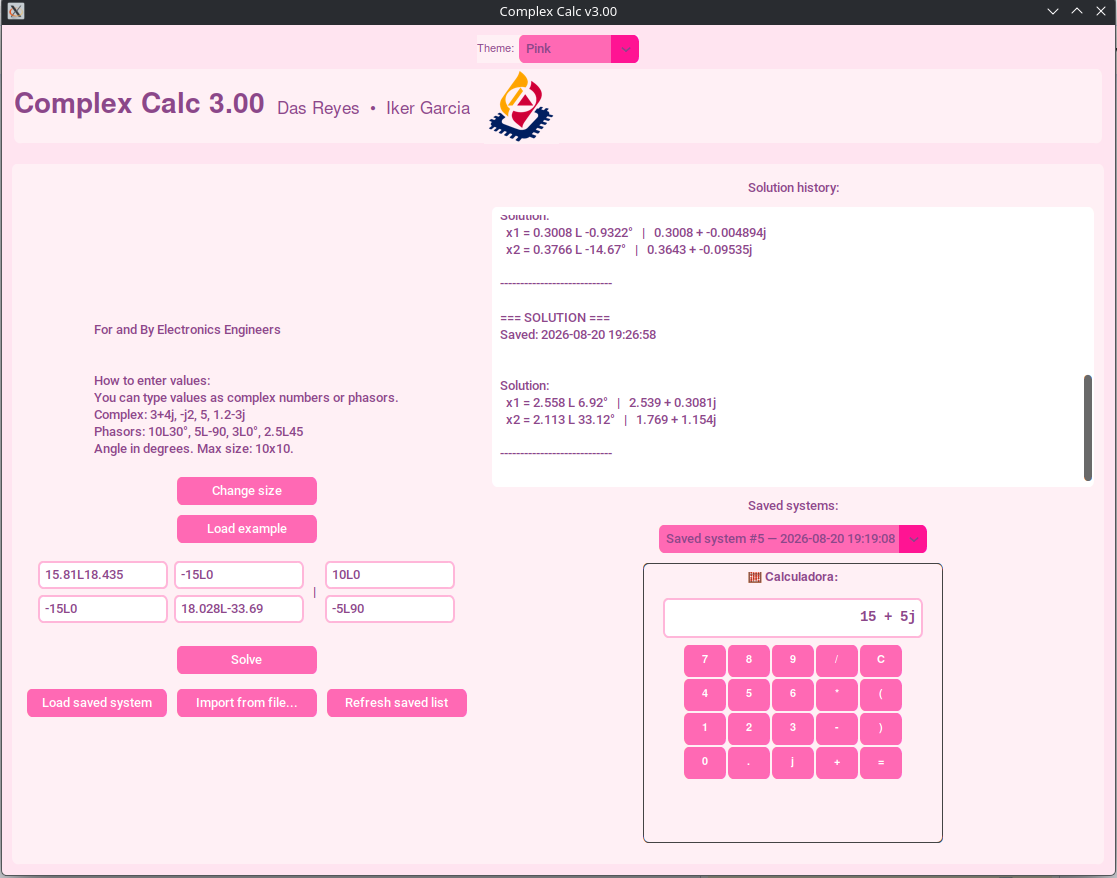
\includegraphics[width=0.68\linewidth]{../src/SolDC.png}
    \fuente{elaboración propia}
    \caption{Solución de un sistema complejo de forma Polar.}
    \label{fig:interfaz4}
\end{figure}

\section{Discusión}

\subsection{Justificación y aportación de la herramienta}

Esta calculadora fue desarrollada con el propósito de facilitar la resolución de sistemas de ecuaciones lineales, tanto con números reales como complejos, y de servir como apoyo en actividades académicas relacionadas con el análisis de circuitos eléctricos. La herramienta permite representar resultados en forma rectangular y polar, lo cual es especialmente útil en cursos como Análisis de Circuitos, Electrónica, Señales y Sistemas y Métodos Matemáticos para la Ingeniería, donde el manejo de cantidades fasoriales es fundamental. \\

Se incorporó un historial para conservar las operaciones realizadas y evitar la pérdida de información durante la resolución de ejercicios. Además, la interfaz fue diseñada para optimizar el tiempo de trabajo del usuario mediante una interacción clara y eficiente. Al ser una herramienta gratuita y ejecutarse en cualquier equipo con Windows / Linux, se convierte en una alternativa accesible dentro del ámbito académico, contribuyendo a la comprensión y visualización de magnitudes complejas mediante su conversión automática entre formas.

\subsection{Proceso de diseño y desarrollo}

Durante el desarrollo del proyecto se presentaron diversos retos. El primero consistió en el diseño de una interfaz lo suficientemente intuitiva para usuarios sin experiencia previa con herramientas de cálculo de números complejos. Las primeras versiones incluían instrucciones dentro de la ventana principal; sin embargo, esto afectaba la claridad visual, por lo que se realizó una reorganización estructural que permitió presentar la información de manera más ordenada y profesional. \\

Asimismo, se presentaron dificultades al implementar las funciones de almacenamiento y carga de matrices. Los errores iniciales durante las pruebas fueron corregidos mediante ajustes en la gestión de archivos y memoria, garantizando así un manejo estable de la información ingresada por el usuario. \\

Finalmente, se detectaron limitaciones en la personalización visual de Tkinter, dado que la aplicación de temas y combinaciones de colores no es directa. Para alcanzar la estética requerida fue necesario modificar de forma manual el archivo \texttt{.json} correspondiente, lo que permitió obtener una interfaz más coherente con el propósito académico del proyecto.


\section{Conclusiones}

El desarrollo de este proyecto permitió comprobar que las herramientas de inteligencia artificial pueden ser útiles durante la programación si se utilizan como apoyo y no como sustituto del conocimiento del programador. A pesar de contar únicamente con conocimientos básicos de C para microcontroladores, fue posible desarrollar una aplicación funcional para resolver sistemas de ecuaciones con números complejos, aplicados al análisis de circuitos. La revisión y las pruebas realizadas durante el desarrollo fueron necesarias para comprobar que el código generado funcionara correctamente y se ajustara a lo que requería el proyecto. \\

En cuanto al resultado técnico, se obtuvo una herramienta que permite trabajar con sistemas de ecuaciones de una forma más práctica que algunos de los métodos utilizados inicialmente. La aplicación permite introducir números complejos tanto en forma rectangular como polar y realizar la conversión entre ambas representaciones utilizando NumPy. También se consiguió generar un ejecutable que facilita su distribución y uso en diferentes equipos, evitando que sea necesario configurar todo el entorno de programación para utilizar la herramienta. \\

Durante el desarrollo también se reforzaron conocimientos relacionados con el álgebra lineal y su aplicación a circuitos eléctricos, principalmente en la representación de sistemas mediante matrices y en la utilización de matrices de impedancias. Una de las principales conclusiones del proyecto fue que utilizar IA para generar o modificar partes del código puede reducir considerablemente el tiempo de desarrollo, pero es necesario entender lo que hace el programa y comprobar cada parte antes de incorporarla. De esta forma, la IA funciona como una herramienta de apoyo, mientras que las decisiones y la validación del resultado siguen dependiendo del desarrollador. \\

Finalmente, el proyecto se publicó utilizando una licencia MIT, por lo que el código puede ser utilizado, estudiado y modificado por otros estudiantes. Aunque la aplicación surgió para resolver una necesidad específica dentro del curso, su estructura permite utilizarla como punto de partida para realizar mejoras o desarrollar herramientas similares. Esto también permite que el proyecto tenga una utilidad más allá de su entrega y que pueda seguir desarrollándose posteriormente.

\begin{thebibliography}{99}

\bibitem{anton}
Anton, H., Rorres, C. \textit{Álgebra lineal con aplicaciones}. Wiley, 2013.

\bibitem{lay}
Lay, D. C. \textit{Álgebra lineal y sus aplicaciones}. 4.ª ed., Pearson, 2012.

\bibitem{numpy}
NumPy Developers. \textit{numpy.linalg.solve — NumPy v2.5 Manual}. NumPy Documentation, 2026. Disponible en: \url{https://numpy.org/doc/stable/reference/generated/numpy.linalg.solve.html}

\bibitem{python}
Python Software Foundation. \textit{Built-in Types — Numeric Types}. Python Documentation, 2026. Disponible en: \url{https://docs.python.org/3/library/stdtypes.html}

\bibitem{tkinter}
Python Software Foundation. \textit{tkinter — Python interface to Tcl/Tk}. Python Documentation, 2026. Disponible en: \url{https://docs.python.org/3/library/tkinter.html}

\bibitem{pyinstaller}
Cortesi, D., Bajo, G., McMillan, W. \textit{PyInstaller Manual}. PyInstaller Documentation, 2026. Disponible en: \url{https://pyinstaller.org/en/stable/}

\bibitem{openai}
OpenAI. \textit{ChatGPT}. OpenAI, 2026. Disponible en: \url{https://chatgpt.com/}

\end{thebibliography}


\end{document}1
